%==============================================================================
%== template for LATEX poster =================================================
%==============================================================================
%
%--A0 beamer slide-------------------------------------------------------------
\documentclass[final]{beamer}
\usepackage[orientation=portrait,size=a0,
            scale=1.25         % font scale factor
           ]{beamerposter}
           
\geometry{
  hmargin=2.5cm, % little modification of margins
}

%
\usepackage[utf8]{inputenc}

\linespread{1.15}
%
%==The poster style============================================================
\usepackage{ulem}
\usetheme{sharelatex}

\usepackage{svg}
\usepackage{alltt}
%https://www.sharelatex.com/learn/Code_listing
%\usepackage{listings}

% Preserve spaces after \newcommand{}
% https://tex.stackexchange.com/a/17873
\usepackage{xspace}

\newcommand{\JournalPaper} {paper in Astronomy & Computing\cite{docker-paper} \xspace}
\newcommand{\ConferencePaper} {conference paper\xspace}

%==Title, date and authors of the poster=======================================
\title
[ADASS Santiago de Chile, Chile, October 22-26, 2017] % Conference
{ % Poster title
Use of Docker for deployment and testing of astronomy software
}

\author{ % Authors
S. Voutsinas\inst{1}, D. Morris\inst{1}, N.C.~Hambly\inst{1}, R.G. Mann\inst{1}
}
\institute
[Institute for Astronomy, School of Physics and Astronomy, University of Edinburgh] % General University
{
\inst{1} Institute for Astronomy, School of Physics and Astronomy, University of Edinburgh
}
\date{\today}



\begin{document}
\begin{frame}[t]
%==============================================================================
\begin{multicols}{3}
%==============================================================================
%==The poster content==========================================================
%==============================================================================

\section{Introduction}

Recent years have seen an explosion of interest in operating system level virtualization, A lot of the activity in this field has centred on Docker and this paper presents lessons learned from two projects we have conducted involving Docker: a simple test of its capabilities as a deployment system and as part of more complicated project connecting a range of Virtual Observatory \cite{vo} services running in separate Docker containers. 



\vskip1ex
\begin{figure}
\centering
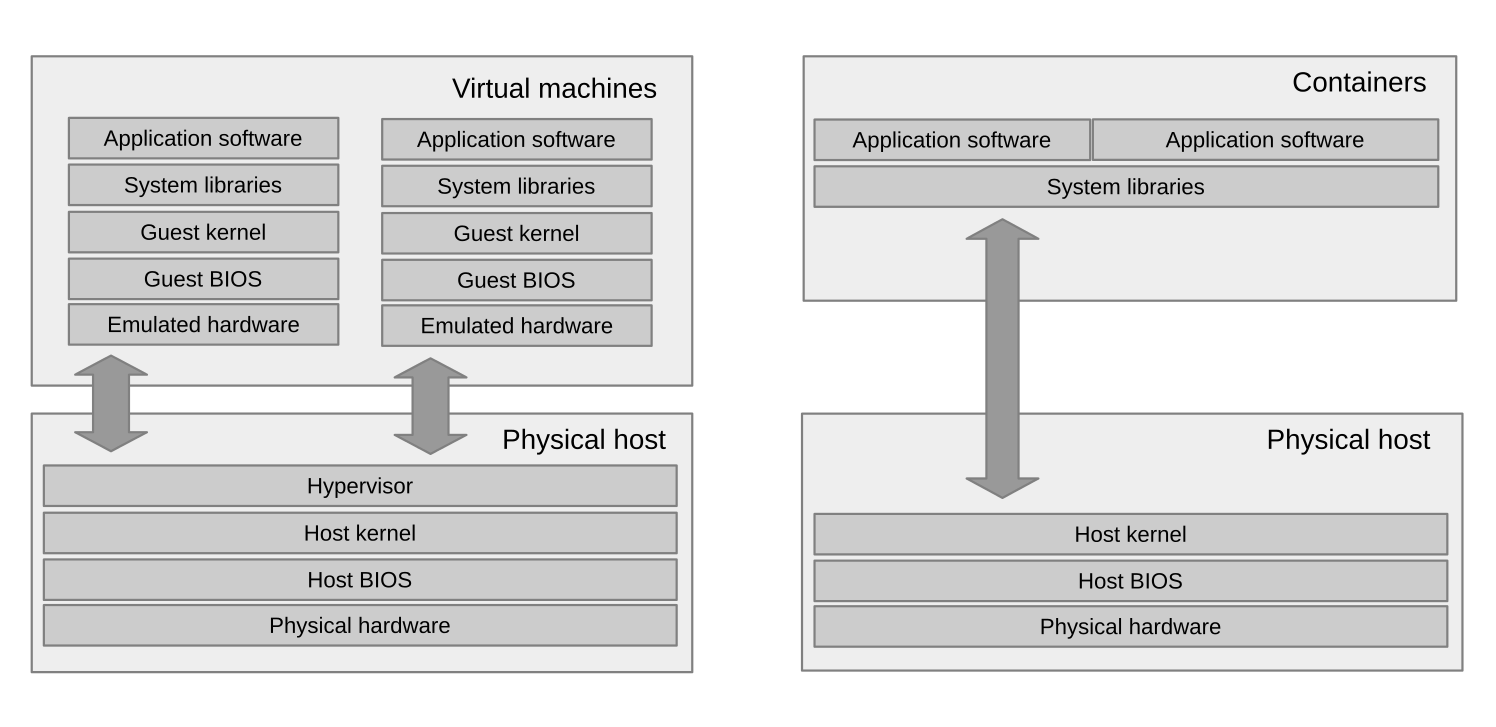
\includegraphics[width=0.99\columnwidth]{virt-layers-001.png}
\caption{Comparison between hardware (left) and operating system level virtualization (right).}
\end{figure}
\vskip2ex


Many of the issues we described in our \JournalPaper have since been solved as the Docker engine and toolset have continued to evolve, but we believe there remains virtue in recounting them, both because they illustrate basic properties of Docker containers and because they show how the Docker community operates. 


\section{Using Docker for desktop applications}
\subsection{IVOATEX in Docker}

As an early experiment in using containers to deploy applications, we used Docker to wrap the IVOAX\cite{ivoatex} document build system to make it easier to use. The IVOATEX system uses a combination of LATEX tools and libraries, a compiled C program to handle LATEX to HTML conversion, and a makefile to manage the build process.

Installing and configuring all of the required components is a complicated process for someone who just wants to make a small edit to an existing IVOA document. In order to address this we created a simple Docker container that incorporates all of the components needed to run the IVOATEX system configured and ready to run.

The output of this is a simple Dockerfile, which anyone with a Docker installation can use to build and use on any environment.

\hfill 

It should be noted that while exploring during this project we encountered a security vulnerability which potentially allows root access to the host file system, unless a fix is applied which changes the user id before running the target application. Since our experiments, newer technologies such as Singularity have been developed, which are better suited for use cases involving desktop applications where the complexity of virtual networking and filesystem that Docker provides is not needed. 


%The source code for our IVOATEX container is available on GitHub and a binary image is available from the Docker registry. 
\hfill \break

%\begin{lstlisting}
%
%    docker run -it
%        -e "useruid=\$(id -u)"
%        -v "\$(pwd):/var/local/texdata"
%        'ivoa/ivoatex'
%
%        make clean
%        make biblio
%        make
%
%\end{lstlisting}

\begin{verbatim}

docker run -it \textbackslash

    -e "useruid=\$(id -u)" \textbackslash
    
    -v "\$(pwd):/var/local/texdata" \textbackslash
    
    'ivoa/ivoatex'

    make clean
    
    make biblio
    
    make

\end{verbatim}

The ivoatex container enables the user to install and run the document build in a few simple commands, as seen in the above example.

\section{Using Docker for service deployment}
\subsection{Firethorn}

The Firethorn project enables users to run queries and store results from local astronomy archive or remote TAP services and share these results with others by publishing them via a local TAP service. The project has its origins in a prototype data resource federation service and is built around the Open Grid Service Architecture Data Access Infrastructure\cite{ogsa-dai}.
A schematic representation of the architecture is shown in (Figure~\ref{fig:firethorn}).

We used Docker both in testing and production, wrapping our Java/Tomcat web services, testing suite and web application in Docker containers.
In our \JournalPaper we cover topics such as how we built our base images, how we managed network connections between the different components and describe the issues we encountered.

\vskip1ex
\begin{figure}
\centering
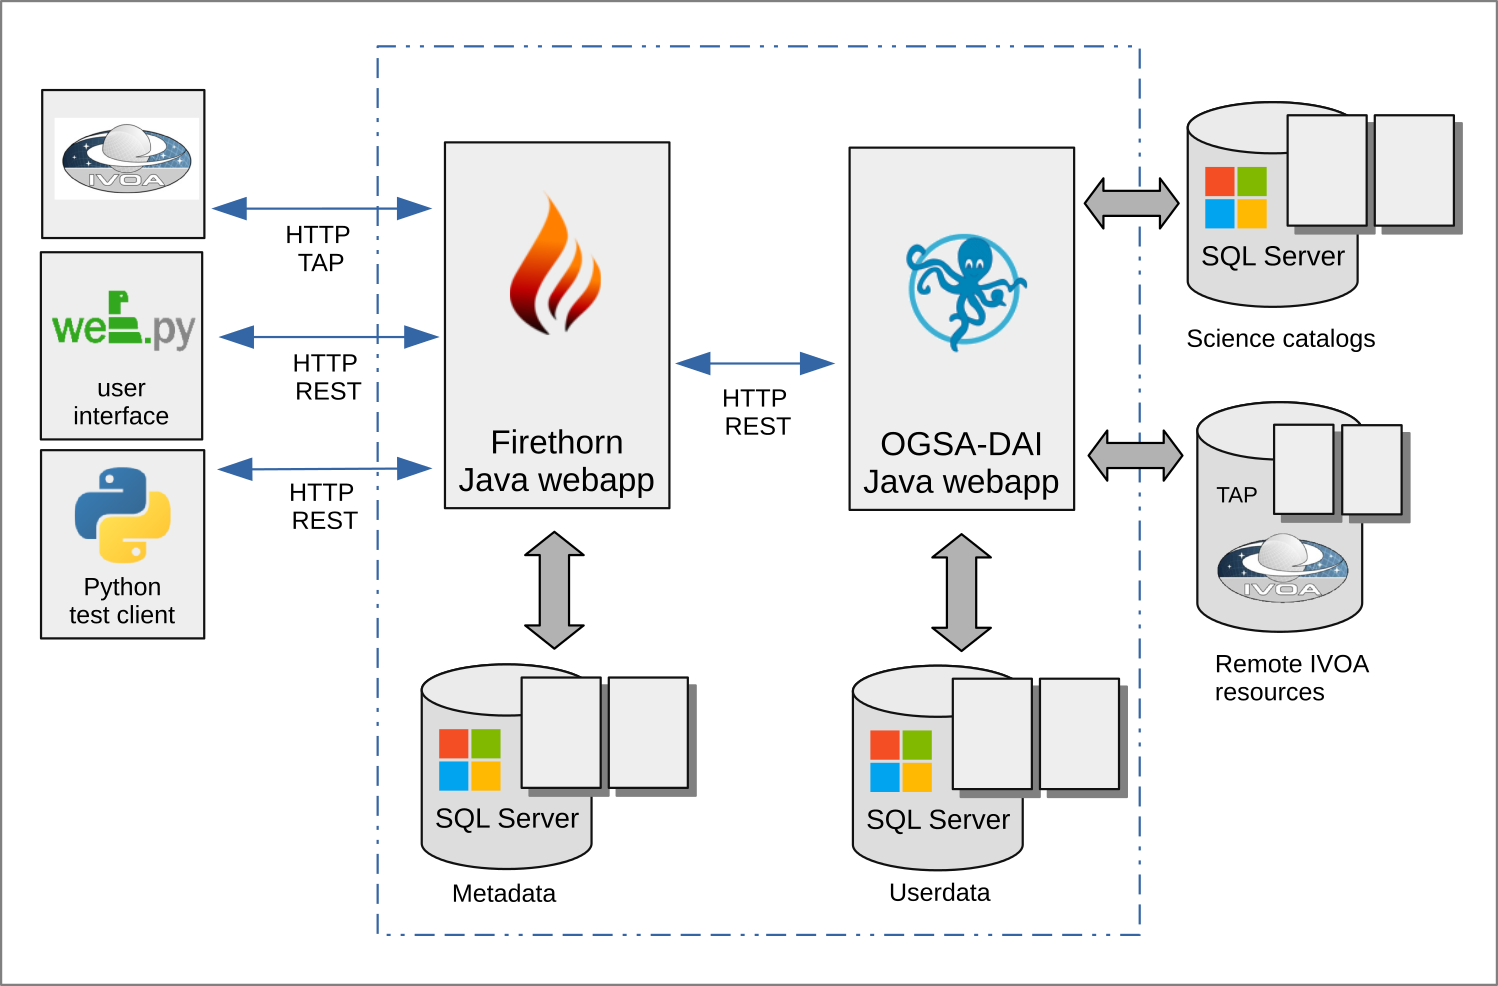
\includegraphics[width=0.99\columnwidth]{docker-chain-000.png}
\caption{Firethorn architecture illustrating the key components and web services.\label{fig:firethorn}}
\end{figure}
\vskip2ex

\section{Using Docker for software development}

One of the key reasons for choosing Docker to deploy our systems was to be able to deploy the software reliably and repeatably on a range of different platforms. 

% In our project the software has to be able to run on a number of % % different platforms, including the developer’s desktop computer, the % integration test systems and at least two different live deployment  environments. 

If we relied on manual configuration for the target platform and runtime environment, then over time it is inevitable that they will end up being slightly different.

In our \JournalPaper we described how we used shell scripts to automate building and running our Docker images, in our \ConferencePaper we bring this up to date describing how our migration to  using docker-compose to orchestrate sets of containers. 

% \sout{In our case, we knew that although we had control over the environment for our own deployments, we would not have the same level of control over deployments at third party sites, which is why achieving automation using configuration management tools such as Puppet or Chef was not applicable.}

% how did we do it ?    
% did it work ?
% what did we learn ?
% what has changed since ?

\vskip1ex
\begin{figure}
\centering
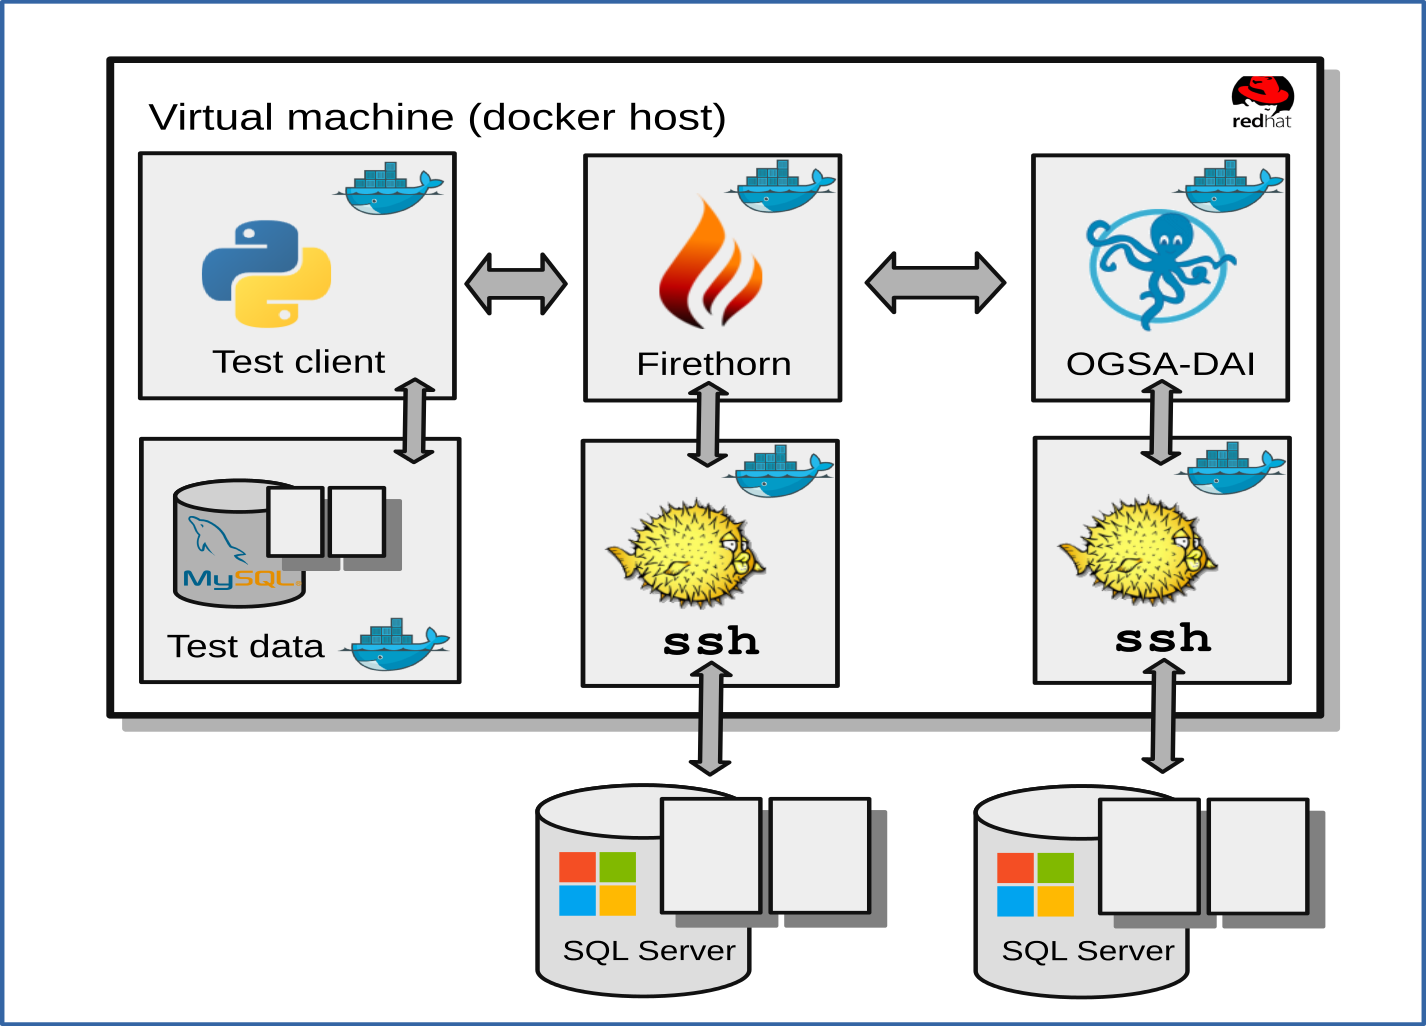
\includegraphics[width=0.99\columnwidth]{docker-chain-ssh.png}
\caption{Interconnected web service containers. \label{fig:containers}}
\end{figure}
\vskip2ex

\section{Summary and conclusions}

From our experience, Docker provides:

\begin{itemize}
  \item Ease in bundling components together
  \item Re-usability, maintainability and faster continuous integration environments 
  \item  Improved collaboration between developers (Dockerfile)
  \item  Openness and Docker Community
  \item  Reproducibility
\end{itemize}


Based on our experience in development and production for the Firethorn and IVOATEX projects, we anticipate a rapid growth of interest and usage of Docker and container-based solutions in general. We expect that this will be the case for both developing and deploying systems as a replacement or complementary to existing hardware virtualization technologies, in enabling reproducible science and in systems that allow scientists to submit their own code to data centres. Docker can potentially help with this, as it provides the tools and simplicity that scientists need to recreate the environment that was used to generate a set of results. 

%==============================================================================
%==End of content==============================================================
%==============================================================================

%--References------------------------------------------------------------------

\subsection{References}

  \begin{thebibliography}{1}

  \bibitem{docker-paper} D. Morris, S. Voutsinas, N.C. Hambly, R.G. Mann, 2017. 
  Use of Docker for deployment and testing of astronomy software. URL: https://arxiv.org/abs/1707.03341

  \bibitem{vo} Arviset, C., Gaudet, S., The IVOA Architecture, Version 1.0, IVOA Note, 23 November 2010. URL: http://www.ivoa.net/documents/Notes/IVOAArchitecture/index.html

  \bibitem{ogsa-dai} Holliman, M., Alemu, T., Hume, A., van Hemert, J., Mann, R.G., Noddle, K., Valkonen, L. Service Infrastructure for Cross-Matching Distributed Datasets Using OGSA-DAI and TAP. In: Evans, I.N., Accomazzi, A., Mink, D.J., Rots, A.H. (Eds.), Astronomical Data Analysis Software and Systems XX. In: Astronomical Society of the Pacific Conference Series, vol. 442, p. 579.

  \bibitem{ivoatex} Demleitner, M., Taylor, M., Harrision, P., Molinaro, M. The IVOATEX Document Preparation System, Version 1.1, IVOA Note, 30
April 2016. URL: http://ivoa.net/documents/Notes/IVOATex/index.html

  \end{thebibliography}
  
%--End of references-----------------------------------------------------------


\begin{figure}
\subfigure{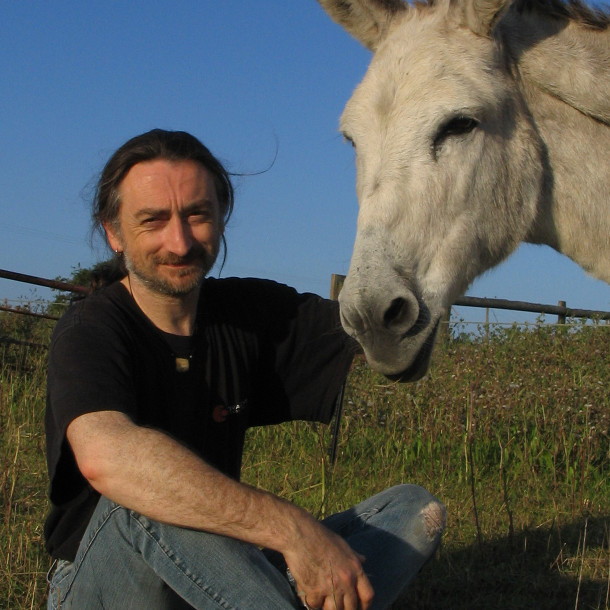
\includegraphics[width=70mm,scale=1.5]{DaveProfileSquare.jpg}}
\hfill
\subfigure{
\includegraphics[width=90mm,scale=1.5]{stelios-img.jpg}}
\hfill
\caption{Dave Morris (left), Stelios Voutsinas (right)}
\end{figure}


\end{multicols}

%==============================================================================
\end{frame}
\end{document}
